\documentclass[11pt,a4paper]{article}

\usepackage[utf8]{inputenc}
\usepackage[T1]{fontenc}
\usepackage{pgfplots} % Required for creating plots
\pgfplotsset{compat=1.17} % Set the compatibility level of pgfplots

\title{Document with pgfplots Examples}
\author{Your Name}
\date{\today}

\begin{document}
	
	\maketitle
	
	\section{Bar Plot Example}
	Next, we present a bar plot.
	
	% Bar plot
	\begin{figure}[h]
		\centering
		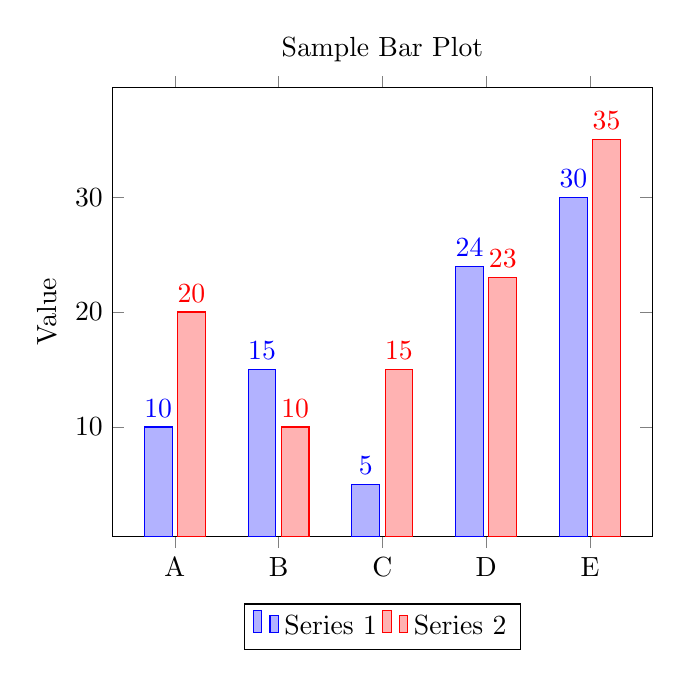
\begin{tikzpicture}
			\begin{axis}[
				title={Sample Bar Plot},
				ybar,
				enlargelimits=0.15,
				legend style={at={(0.5,-0.15)},
					anchor=north,legend columns=-1},
				ylabel={Value},
				symbolic x coords={A, B, C, D, E},
				xtick=data,
				nodes near coords,
				nodes near coords align={vertical},
				]
				\addplot coordinates {(A,10) (B,15) (C,5) (D,24) (E,30)};
				\addplot coordinates {(A,20) (B,10) (C,15) (D,23) (E,35)};
				\legend{Series 1, Series 2}
			\end{axis}
		\end{tikzpicture}
		\caption{A simple bar plot}
	\end{figure}

\section{Scatter Plot Example}
A scatter plot representing some data points is shown below.

% Scatter plot
\begin{figure}[h]
	\centering
	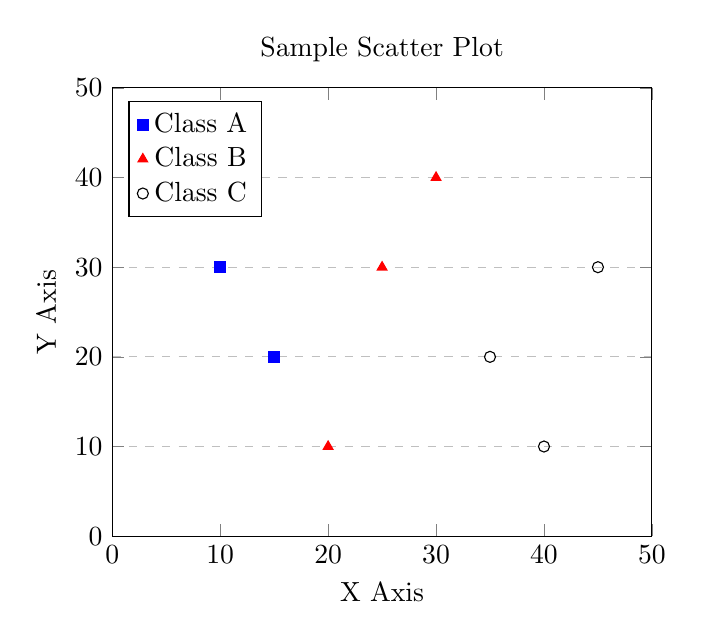
\begin{tikzpicture}
		\begin{axis}[
			title={Sample Scatter Plot},
			xlabel={X Axis},
			ylabel={Y Axis},
			xmin=0, xmax=50,
			ymin=0, ymax=50,
			legend pos=north west,
			ymajorgrids=true,
			grid style=dashed,
			]
			
			% Adding a scatter plot
			\addplot[
			scatter, % Enables scatter plot
			only marks, % Only points, no lines
			point meta=explicit symbolic, % Allows for custom labels
			scatter/classes={
				a={mark=square*,blue}, % Style for class 'a'
				b={mark=triangle*,red}, % Style for class 'b'
				c={mark=o,draw=black,fill=black} % Style for class 'c'
			},
			]
			table[meta=label]{
				x   y   label
				5   40  a
				10  30  a
				15  20  a
				20  10  b
				25  30  b
				30  40  b
				35  20  c
				40  10  c
				45  30  c
			};
			\legend{Class A, Class B, Class C}
			
		\end{axis}
	\end{tikzpicture}
	\caption{A simple scatter plot with different point styles}
\end{figure}
\end{document}
